\documentclass[a4paper,12pt]{article}
\usepackage{xcolor}
\usepackage{amsmath,amsfonts,amssymb}
\usepackage{geometry}
\usepackage{fancyhdr}
\usepackage{graphicx}
\usepackage{titlesec}
\usepackage{tikz}
\usepackage{booktabs}
\usepackage{array}
\usetikzlibrary{shadows}
\usepackage{tcolorbox}
\usepackage{float}
\usepackage{lipsum}
\usepackage{mdframed}
\usepackage{pagecolor}
\usepackage{mathpazo}   % Palatino font (serif)
\usepackage{microtype}  % Better typography
\usepackage{subfigure}
% \hypersetup{
%   colorlinks=true,
%   linkcolor=blue,
%   urlcolor=blue,
%   citecolor=blue
% }

% Page background color
\pagecolor{gray!10!white}

% Geometry settings
\geometry{margin=0.5in}
\pagestyle{fancy}
\fancyhf{}

% Fancy header and footer
\fancyhead[C]{\textbf{\color{blue!80}CS754 Assignment-4}}
% \fancyhead[R]{\color{blue!80}Saksham Rathi}
\fancyfoot[C]{\thepage}

% Custom Section Color and Format with Sans-serif font
\titleformat{\section}
{\sffamily\color{purple!90!black}\normalfont\Large\bfseries}
{\thesection}{1em}{}

% Custom subsection format
\titleformat{\subsection}
{\sffamily\color{cyan!80!black}\normalfont\large\bfseries}
{\thesubsection}{1em}{}

% Stylish Title with TikZ (Enhanced with gradient)
\newcommand{\cooltitle}[1]{%
  \begin{tikzpicture}
    \node[fill=blue!20,rounded corners=10pt,inner sep=12pt, drop shadow, top color=blue!50, bottom color=blue!30] (box)
    {\Huge \bfseries \color{black} #1};
  \end{tikzpicture}
}
\usepackage{float} % Add this package

\newenvironment{solution}[2][]{%
    \begin{mdframed}[linecolor=blue!70!black, linewidth=2pt, roundcorner=10pt, backgroundcolor=yellow!10!white, skipabove=12pt, skipbelow=12pt]%
        \textbf{\large #2}
        \par\noindent\rule{\textwidth}{0.4pt}
}{
    \end{mdframed}
}

% Document title
\title{\cooltitle{CS754 Assignment-4}}
\author{{\bf Saksham Rathi, Ekansh Ravi Shankar, Kshitij Vaidya}}
\date{}

\begin{document}
\maketitle
\textbf{Declaration:} The work submitted is our own, and
we have adhered to the principles of academic honesty while completing and submitting this work. We have not referred to any unauthorized sources, and we have not used generative AI tools for the work submitted here.

\section*{Question 1}

\begin{solution}{Solution}
  \section{Experimental Results}

  We generated a sensing matrix over a Bernoulli Distribution and a sparse signal over a Uniform Distribution. We then reconstruct the sparse signal using the CVZ package in MATLAB. The results are shown in figures \ref{fig:validationError} and \ref{fig:rmse}. From the plots for VE and RMSE, we can see that they follow similar shapes and trends for different values of sparsity. This means that our hypothesis that the validation error is a good proxy for the RMSE is correct. From the plots, the optimal value of $\lambda$ is in the range of $5-10$.
  \begin{enumerate}
  \item \textbf{Shape of the Plots} : Both the plots have a U-shaped curve. For very small values of $\lambda$, the model is underfitting, leading to high validation error and RMSE. As $\lambda$ increases, the model complexity decreases, leading to lower validation error and RMSE. However, after a certain point, increasing $\lambda$ leads to overfitting, causing both metrics to increase again.

  \item \textbf{Effect of Sparsity} : We expect that as the sparsity increases, the values of the validation error and RMSE to be higher for sparser signals, as they are harder to reconstruct accurately. This trend is not quite exactly followed but we can attribute this to the randomness in the generation of the sensing matrix. But the overall trend and the choice of $\lambda$ is still valid.
  \end{enumerate}

  \section{Effect of $\mathcal{V} = \mathcal{R}$ in Compressive Sensing}

  When the validation set $\mathcal{V}$ is equal to the training set $\mathcal{R}$, the theoretical guarantees and practical utility of the cross-validation in Compressive Sensing collapse.

  \subsection{Breakdown of Statistical Assumptions}

  The paper's analysis assumes that the training and validation sets are independent. When $\mathcal{V} = \mathcal{R}$ and the sets become coincident:

  \begin{enumerate}
    \item \textbf{Loss of Independence} : The Cross Validation residual $\epsilon_{\text{cv}} = \| \mathbf{y}_{cv} - \mathbf{A}_{cv} \hat{\mathbf{x}} \|_2^2$ uses the same measurements as the  ($\mathbf{y}_{cv} = \mathbf{y}$, $\mathbf{A}_{cv} = \mathbf{A}$) reconstruction. This violates the statistical independence required for unbiased error estimation.
    \item \textbf{Overfitting Risk} : The reconstruction algorithm minimizes $\| \mathbf{y} - \mathbf{A} \hat{\mathbf{x}} \|_2^2$. If $ V = R $, $\epsilon_{\text{cv}}$ reflects a zero training error not a generalisation error leading to overfitting. The CV residual becomes a biased optimistic estimate of the true error $\varepsilon_{\mathbf{x}}$
  \end{enumerate}

  \subsection{Theoretical Guarantees Fail}

  The results from Lemma 1 and Theorem 1 rely on the independence of the training and validation sets. When $\mathcal{V} = \mathcal{R}$, the guarantees provided by these lemmas and theorems become invalid. The bounds on the expected error and the convergence rates are no longer applicable, as they depend on the assumption of independent samples.

  \begin{enumerate}
    \item \textbf{Lemma 1 : CV Residual Distribution} : The distribution $\epsilon_{\text{cv}} \sim \mathcal{N}\left(\mu, \sigma^2\right)$ assumes independence of $\mathcal{R}$ and $\mathcal{V}$. When $\mathcal{V} = \mathcal{R}$, the distribution of the CV residual becomes degenerate, leading to unreliable estimates of the mean and variance because the Central Limit Theorem approximation is invalidated.
    \item \textbf{Theorem 1 : Expected Error Bound} : The error bound 
    \begin{align*}
      h(\lambda, \pm) \epsilon_{\text{cv}} - \sigma_{\mathbf{n}}^2 \leq \varepsilon_{\mathbf{x}} \leq h(\lambda, -) \epsilon_{\text{cv}} - \sigma_{\mathbf{n}}^2 
    \end{align*}
    depends on $\epsilon_{\text{cv}}$ being unbiased. When $ V = R $, $\epsilon_{\text{cv}}$ is downward-biased, rendering the bounds meaningless.
  \end{enumerate}


  \section{Justification of CV Residual as Proxy for MSE}

  The proxying ability of cross-validation residuals to estimate the actual mean squared error is addressed in Lemma 1 and Theorem 1 of the paper.

  \subsection{Lemma 1 : CV Residual Distribution}

  The CV residual $\epsilon_{\textbf{cv}}$ is shown to follow a normal distribution parameterised by the true recovery error (MSE) $\varepsilon_{\mathbf{x}}$ and the noise variance $\sigma_{\mathbf{n}}^2$. The lemma states that:
  \begin{align*}
    \epsilon_{\text{cv}} \sim \mathcal{N}\left(\mu, \sigma^2\right),
  \end{align*} 
  where:
  \begin{enumerate}
      \item $\mu = \frac{m_{\text{cv}}}{m} \left(\varepsilon_{\mathbf{x}} + \sigma_{\mathbf{n}}^2\right)$ is the mean,
      \item $\sigma^2 = \frac{2m_{\text{cv}}}{m^2} \left(\varepsilon_{\mathbf{x}} + \sigma_{\mathbf{n}}^2\right)^2$ is the variance,
      \item $\varepsilon_{\mathbf{x}} = \|\mathbf{x} - \hat{\mathbf{x}}\|_2^2$ is the true MSE between the original signal $\mathbf{x}$ and its estimate $\hat{\mathbf{x}}$,
      \item $\sigma_{\mathbf{n}}^2$ is the noise variance,
      \item $m_{\text{cv}}$ and $m$ are the number of CV and reconstruction measurements, respectively.
  \end{enumerate}

  \noindent This implies that the observable CV residual is directly related to the unobservable MSE. The mean of $\epsilon_{\text{cv}}$ scales linearly with $\varepsilon_{\mathbf{x}}$, making it a statistically valid proxy.

  \subsection{Theorem 1 : Probabilistic Bound on Recovery Error}

  The theorem quantifies how tightly $\epsilon_{\text{cv}}$ bounds $\varepsilon_{\mathbf{x}}$ with high probability:
  \begin{align*}
    h(\lambda,+) \epsilon_{\text{cv}} - \sigma_{\mathbf{n}}^2 \leq \varepsilon_{\mathbf{x}} \leq h(\lambda,-) \epsilon_{\text{cv}} - \sigma_{\mathbf{n}}^2,
  \end{align*}
  where:
  \begin{enumerate}
      \item $h(\lambda, \pm) = \displaystyle\frac{m}{m_{\text{cv}}} \displaystyle\frac{1}{1 \pm \lambda \sqrt{\displaystyle\frac{2}{m_{\text{cv}}}}}$ defines the scaling factors,
      \item $\lambda$ controls the confidence level via the error function $\operatorname{erf}(\lambda/\sqrt{2})$,
      \item The bounds hold with probability $\operatorname{erf}(\lambda/\sqrt{2})$, e.g., $\lambda = 3$ corresponds to $99.7\%$ confidence.
  \end{enumerate}

  \subsection{Conclusions}

  \begin{enumerate}
    \item \textbf{Proxy Relationship} : The inequality directly uses $\epsilon_{\text{cv}}$ to bound $\varepsilon_{\mathbf{x}}$, even though $\mathbf{x}$ is unknown. This enables us to estimate recovery quality using only the CV residual.
    \item \textbf{Tightness of Bounds:} The interval width scales as $\mathcal{O}(1/m_{\text{cv}}^{2/3})$, meaning more CV measurements ($m_{\text{cv}}$) tighten the bounds.
  \end{enumerate}

  

  \section{Comparing Cross-Validation and Theoretical $\lambda$}

  \subsection{Theoretical Choice of $\lambda$}

  The theorem in Tshibirani et al. provides a data-independent $\lambda$ under specific assumptions:
  \begin{enumerate}
    \item \textbf{Assumption} : The design matrix $\mathbf{X}$ satisfies the restricted eigenvalue condition over $\mathcal{C}(S;3)$
    \item \textbf{Guarantee} : For $\lambda_N \geq \frac{2\|\mathbf{X}^T \mathbf{w}\|_\infty}{N}$, the Lasso estimate $\hat{\beta}$ satisfies:
    \begin{align*}
      \|\hat{\beta} - \beta^*\|_2 \leq \frac{3}{\gamma} \sqrt{\frac{k}{N}} \lambda_N
    \end{align*}
    where $\gamma > 0$ is the RE parameter, $k$ is the sparsity level, and $\mathbf{w}$ is the noise vector.
  \end{enumerate} 

  \subsection{Cross Validation Choice of $\lambda$}
  Cross Validation (CV) selects $\lambda$ empirically by:
  \begin{enumerate}
      \item Partitioning data into training/validation sets.
      \item Choosing $\lambda$ that minimizes prediction error on the validation set.
  \end{enumerate}

  \subsection{Advantages of CV over Theoretical $\lambda$}
  \begin{enumerate}
      \item \textbf{Adaptability to Data} :
      \begin{enumerate}
          \item Theorem 11.1 assumes the RE condition and knowledge of $\gamma$, which are often unknown in practice. CV requires no such assumptions and adapts $\lambda$ to the observed data.
          \item The theoretical $\lambda$ is conservative (designed for worst-case guarantees), while CV optimizes $\lambda$ for the specific dataset.
      \end{enumerate}

      \item \textbf{Handling Model Mismatch} : If assumptions like exact sparsity or RE condition are violated, the theoretical $\lambda$ may over/under-regularize. CV automatically adjusts to the true signal structure.

      \item \textbf{Practical Performance} : The theoretical $\lambda$ prioritizes statistical guarantees (error bounds), often leading to over-regularization. CV balances prediction accuracy and model complexity, typically achieving lower prediction error in practice.

      \item \textbf{Noise Adaptation} : Theorem 11.1 requires $\lambda_N \propto \|\mathbf{X}^T \mathbf{w}\|_\infty$, which depends on unobserved noise $\mathbf{w}$. CV bypasses this by directly measuring validation error.
  \end{enumerate}

  \subsection{Limitations of Cross Validation}
  \begin{enumerate}
      \item \textbf{Computational Cost} : CV requires fitting the model multiple times, unlike the closed-form $\lambda$ in Theorem 11.1.
      \item \textbf{Theoretical Guarantees} : CV lacks finite-sample error bounds, whereas Theorem 11.1 provides explicit guarantees under its assumptions.
  \end{enumerate}


  \section{Using Mozorov's Criterion for $\lambda$ Selection}
   
  According to the Mozorov criterion, the optimal value of lambda is chosen to minimize the following expression:
  \begin{align*}
    \lambda^* = \arg\min_{\lambda} | \|\mathbf{y} - \Phi \hat{\mathbf{x}}\|_2^2 - M * \sigma^2 |
  \end{align*}
  where,
  \begin{enumerate}
    \item M is the number of measurements
    \item $\sigma^2$ is the noise variance
    \item $\mathbf{y}$ is the observed signal
    \item $\Phi$ is the sensing matrix
  \end{enumerate}

  \subsection{Advantages of Mozorov's Criterion}
  \begin{enumerate}
    \item Provides a rigourous criterion based on the noise level which aligns well with the problems where the noise variance is known.
    \item The method is less computationally expensive than cross-validation which needs the data to be split into training and validation sets and solving multiple optimization problems. Since this method uses directly observed data making it faster
    \item The method is more stable where data is scarce or noisy unlike cross validation which can be sensitive to the choice of training and validation splits.
  \end{enumerate}

  \subsection{Disadvantages of Mozorov's Criterion}
  \begin{enumerate}
    \item Requires a more accurate estimation of the noise variance $\sigma^2$ which can be difficult in practice. Otherwise the chosen $\lambda$ may not be optimal leading to either overfitting or insufficient regularisation.
    \item The method does not validate against unseen data so the chosen $\lambda$ may not generalize well to new data.
    \item In supervised learning problems, the goal is prediction accuracy rather than reconstruction, cross validation is preferred since it directly minimises the prediction error.
    \item If the assumed noise model does not match the true noise characteristics, the discrepancy principle may fail to choose the optimal $\lambda$.
  \end{enumerate}

  \subsection{Experimental Results}

  \noindent Similar to Cross Validation, we implemented a MATLAB code to find the optimal value of $\lambda$ using the Mozorov criterion. The results are shown in figure \ref{fig:mozorov}. The optimal value of $\lambda$ is around $5-10$ which is similar to the values obtained from cross validation. This shows that the Mozorov criterion is a good alternative to cross validation for choosing $\lambda$ in the given setup. 

  \section{K-Fold Cross Validation}

  The symbol K in the paper refers to the \textbf{Number of Folds} in the K-fold cross validation. This is the number of partitions the dataset is divided into for training and validation. The parameter $\lambda$ is chosen by minimizing the average prediction error over the K folds. The process is used as it balances the efficiency and reliability of the choice of $\lambda$.
  
  \subsection{Theorem 4.1 : Cross Validated LASSO}
  For any \(\alpha \in (0, 1)\),
  \begin{align*}
  \|\hat{\beta}(\hat{\lambda}) - \beta\|_{2,n} \leq 
  \sqrt{\frac{C s \log(p/\alpha)}{n}} \times 
  \sqrt{\log(pn) + s^{-1} \log^{r+1} n}
  \end{align*}
  with probability at least $1 - \alpha - C n^{-c}$, where $c, C > 0$ are constants depending only on $c_1, C_1, K, a, q,$ and $r$.

  \noindent The paper also claims that the cross validated LASSO estimator has the fastest possible rate of convergence in the prediction norm upto a small factor. 

  \subsection{Key Differences between the Bounds}

  \begin{enumerate}
    \item Choice of Penalty Parameter ($\lambda$) 
    \begin{enumerate}
      \item Tibshirani et al. provides a theoretically determined data independent $\lambda$ that doesn't depend on the noise structure. This is not adaptive and assumes prior knowledge of the noise properties.
      \item The Cross Validation Paper uses data driven K Fold Cross Validation to select $\lambda$. This does not require explicit theoretical constraints or prior knowledge of noise. The method is more practical but introduces additional variability.
    \end{enumerate}

    \item Assumptions Made 
    \begin{enumerate}
      \item Tibshirani et al. relies on the Restricted Eigenvalue condition on the design matrix X ensuring invertibility over sparse vectors. This is a strong geometric assumption.
      \item Cross Validation Paper imposes weaker assumptions like sparsity, moment conditions on covariates like bounded sparse eigenvalues and smooth noise transformations. It avoids the RE condition making the results more generalisable.
    \end{enumerate}
  
  \item Error Bounds
  \begin{enumerate}
    \item Tibshirani et al. achieves an L2 error bound scaling as $\mathcal{O}\left(\displaystyle\frac{k\lambda}{\gamma}\right)$ where $\gamma$ is the RE parameter. This is rate optimal under the RE condition.
    \item The paper derives a prediction error bound of $\mathcal{O}\left(\sqrt{\displaystyle\frac{s\log{p}}{n}}\cdot \sqrt{\log{pn}}\right)$ which is nearly optimal but includes additional logarithmic terms. These terms arise because of the adaptive nature of the method and the high dimensional setting.
  \end{enumerate}

  \item Practicality vs Theoretical Tightness
  \begin{enumerate}
    \item Tibshirani et al. provides a theoretically tight bound but requires knowledge of noise properties and RE conditions which are hard to verify in practice.
    \item Cross Validation sacrifices tightness for adaptivity and broader applicability, accomodating unknown noise and avoiding RE conditions. This makes it more practical for real-world applications.
  \end{enumerate}
  \end{enumerate}

\noindent In conclusion, cross-validated LASSO achieves near-optimal error bounds with weaker assumptions and practical $\lambda$ selection at the cost of logarithmic factors in the error bound. In contrast, Tibshirani's bound is theoretically tighter but relies on stronger assumptions and non-adaptive $\lambda$ selection. The choice between the two methods depends on the specific problem context and the available information about the data.

\end{solution}

\begin{figure}[htbp]
  \centering
  \subfigure[Log Scale]{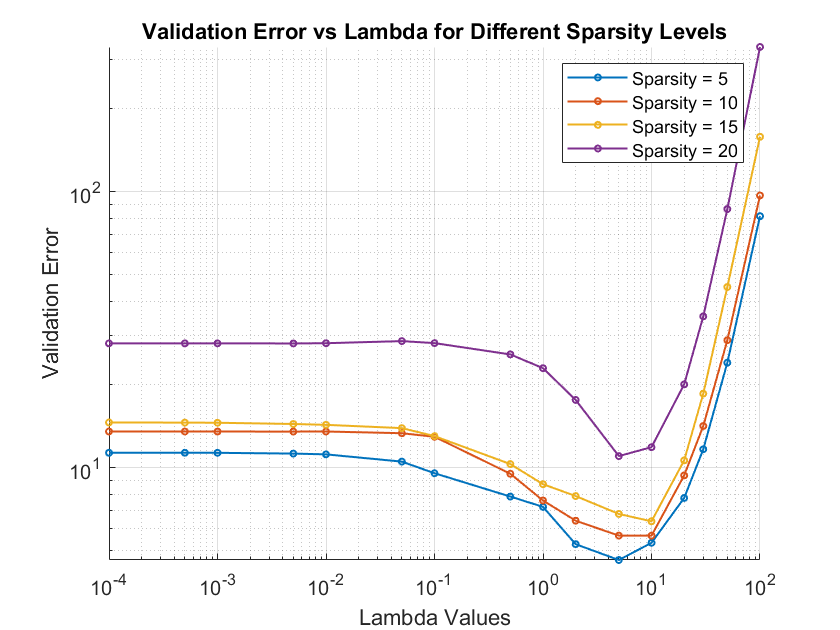
\includegraphics[width=0.45\textwidth]{validationError.png}}
  \subfigure[Linear Scale]{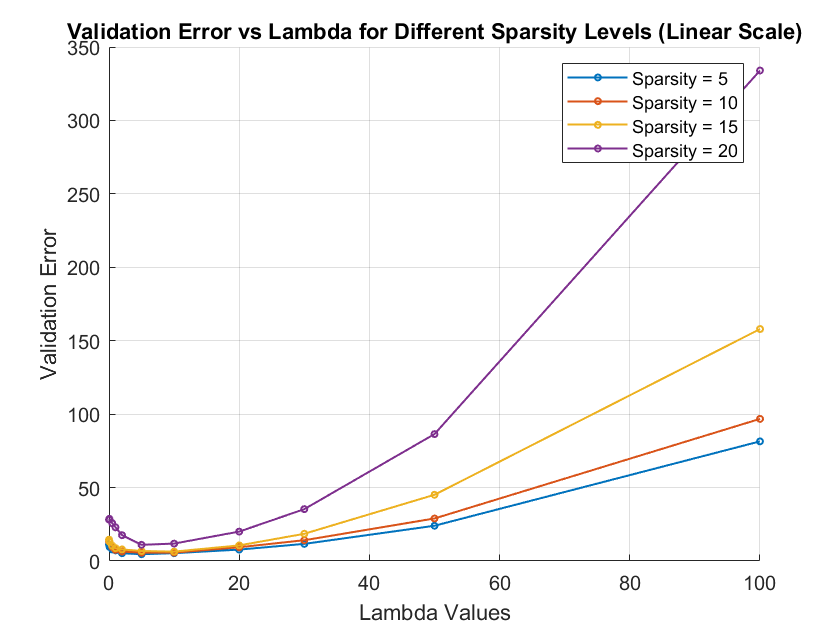
\includegraphics[width=0.45\textwidth]{validationErrorLinear.png}}
  \caption{Validation Error vs. $\lambda$ for different values of sparsity}
  \label{fig:validationError}
\end{figure}

\begin{figure}[htbp]
  \centering
  \subfigure[Log Scale]{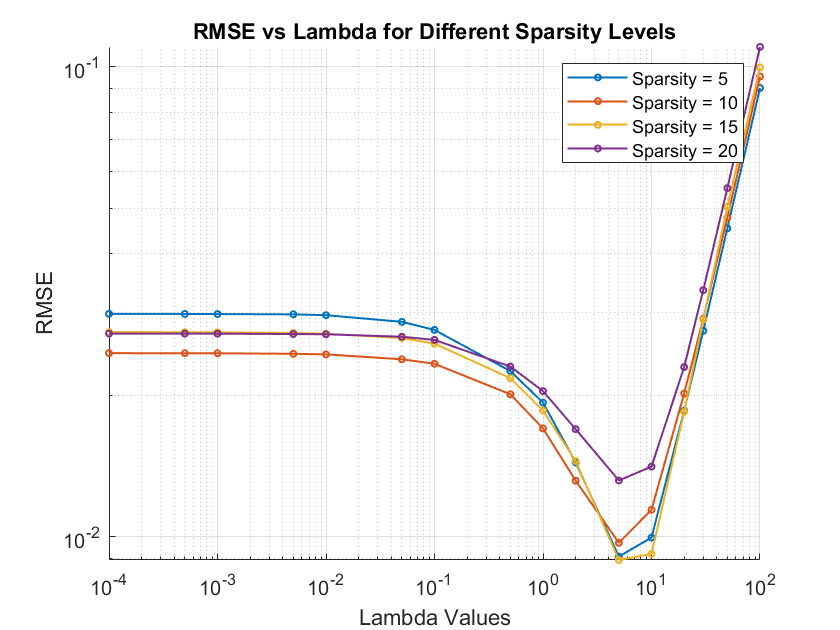
\includegraphics[width=0.45\textwidth]{rmse.png}}
  \subfigure[Linear Scale]{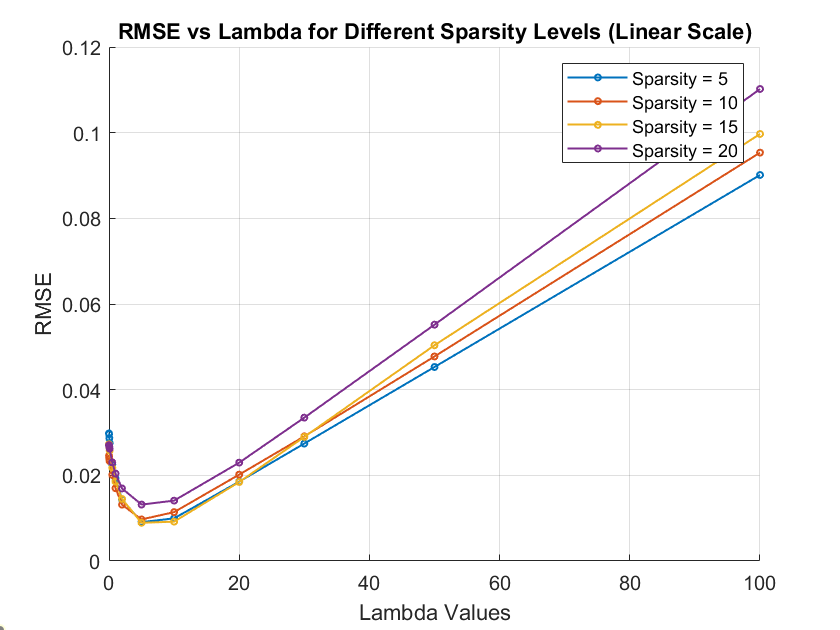
\includegraphics[width=0.45\textwidth]{rmseLinear.png}}
  \caption{RMSE vs. $\lambda$ for different values of sparsity}
  \label{fig:rmse}
\end{figure}

\begin{figure}[htbp]
  \centering
  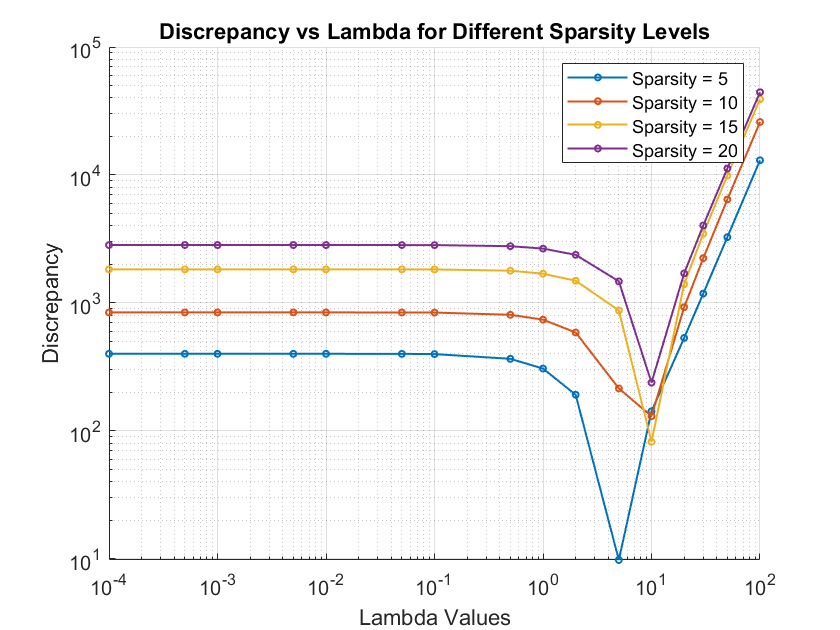
\includegraphics[width=0.45\textwidth]{mozorovCriterion.png}
  \caption{Optimal $\lambda$ using the Mozorov Criterion}
  \label{fig:mozorov}
\end{figure}


\end{document}
